\documentclass[10pt,a4paper]{article}
\usepackage[latin1]{inputenc}
\usepackage{amsthm}
\usepackage{amsmath}
\usepackage{amsfonts}
\usepackage{amssymb}
\usepackage{graphicx}
\usepackage{subfigure}

\newtheorem{theorem}{Theorem}
\newtheorem{corollary}{Corollary}

\begin{document}

\title{Dynamics of Particle Swarm}

\date{}

\maketitle

In order to understand what happens in a PSO(Particle swarm optimization), people are usually interested with the ``exploration and exploitation'' of this algorithm.
\begin{itemize}
\item ``Exploration'' means \textbf{search capability}, which determines how likely the particles could find local best and global best;
\item ``Exploitation'' leads to \textbf{convergence}, which shows how the particles utilize the found current best.
It also tells what happens on the swarm behavior when no new global best can be found.
\end{itemize}

There is no guarantee that PSO could always find a global optimal.
It is not hard to give an example that the global optimal could not be found. 
The factors impact the likelihood that the global optimal is found include:
\begin{itemize}
\item number of particles,
\item $ \chi $, $ \phi^{P} $, $ \phi^{G} $,
\item and the distribution of the fitness space.
\end{itemize}

Our analysis will focus on a standard PSO.
It includes the canonical update rule and a ring topology (single and consistent global best).

Define three types of agents in a particle swarm, which are \emph{particle agent}, \emph{global best agent} and \emph{personal best agent}.
We can have a topology of the swarm in a ring structure, as in Figure \ref{fig:topology3}.

\begin{figure}
\centering
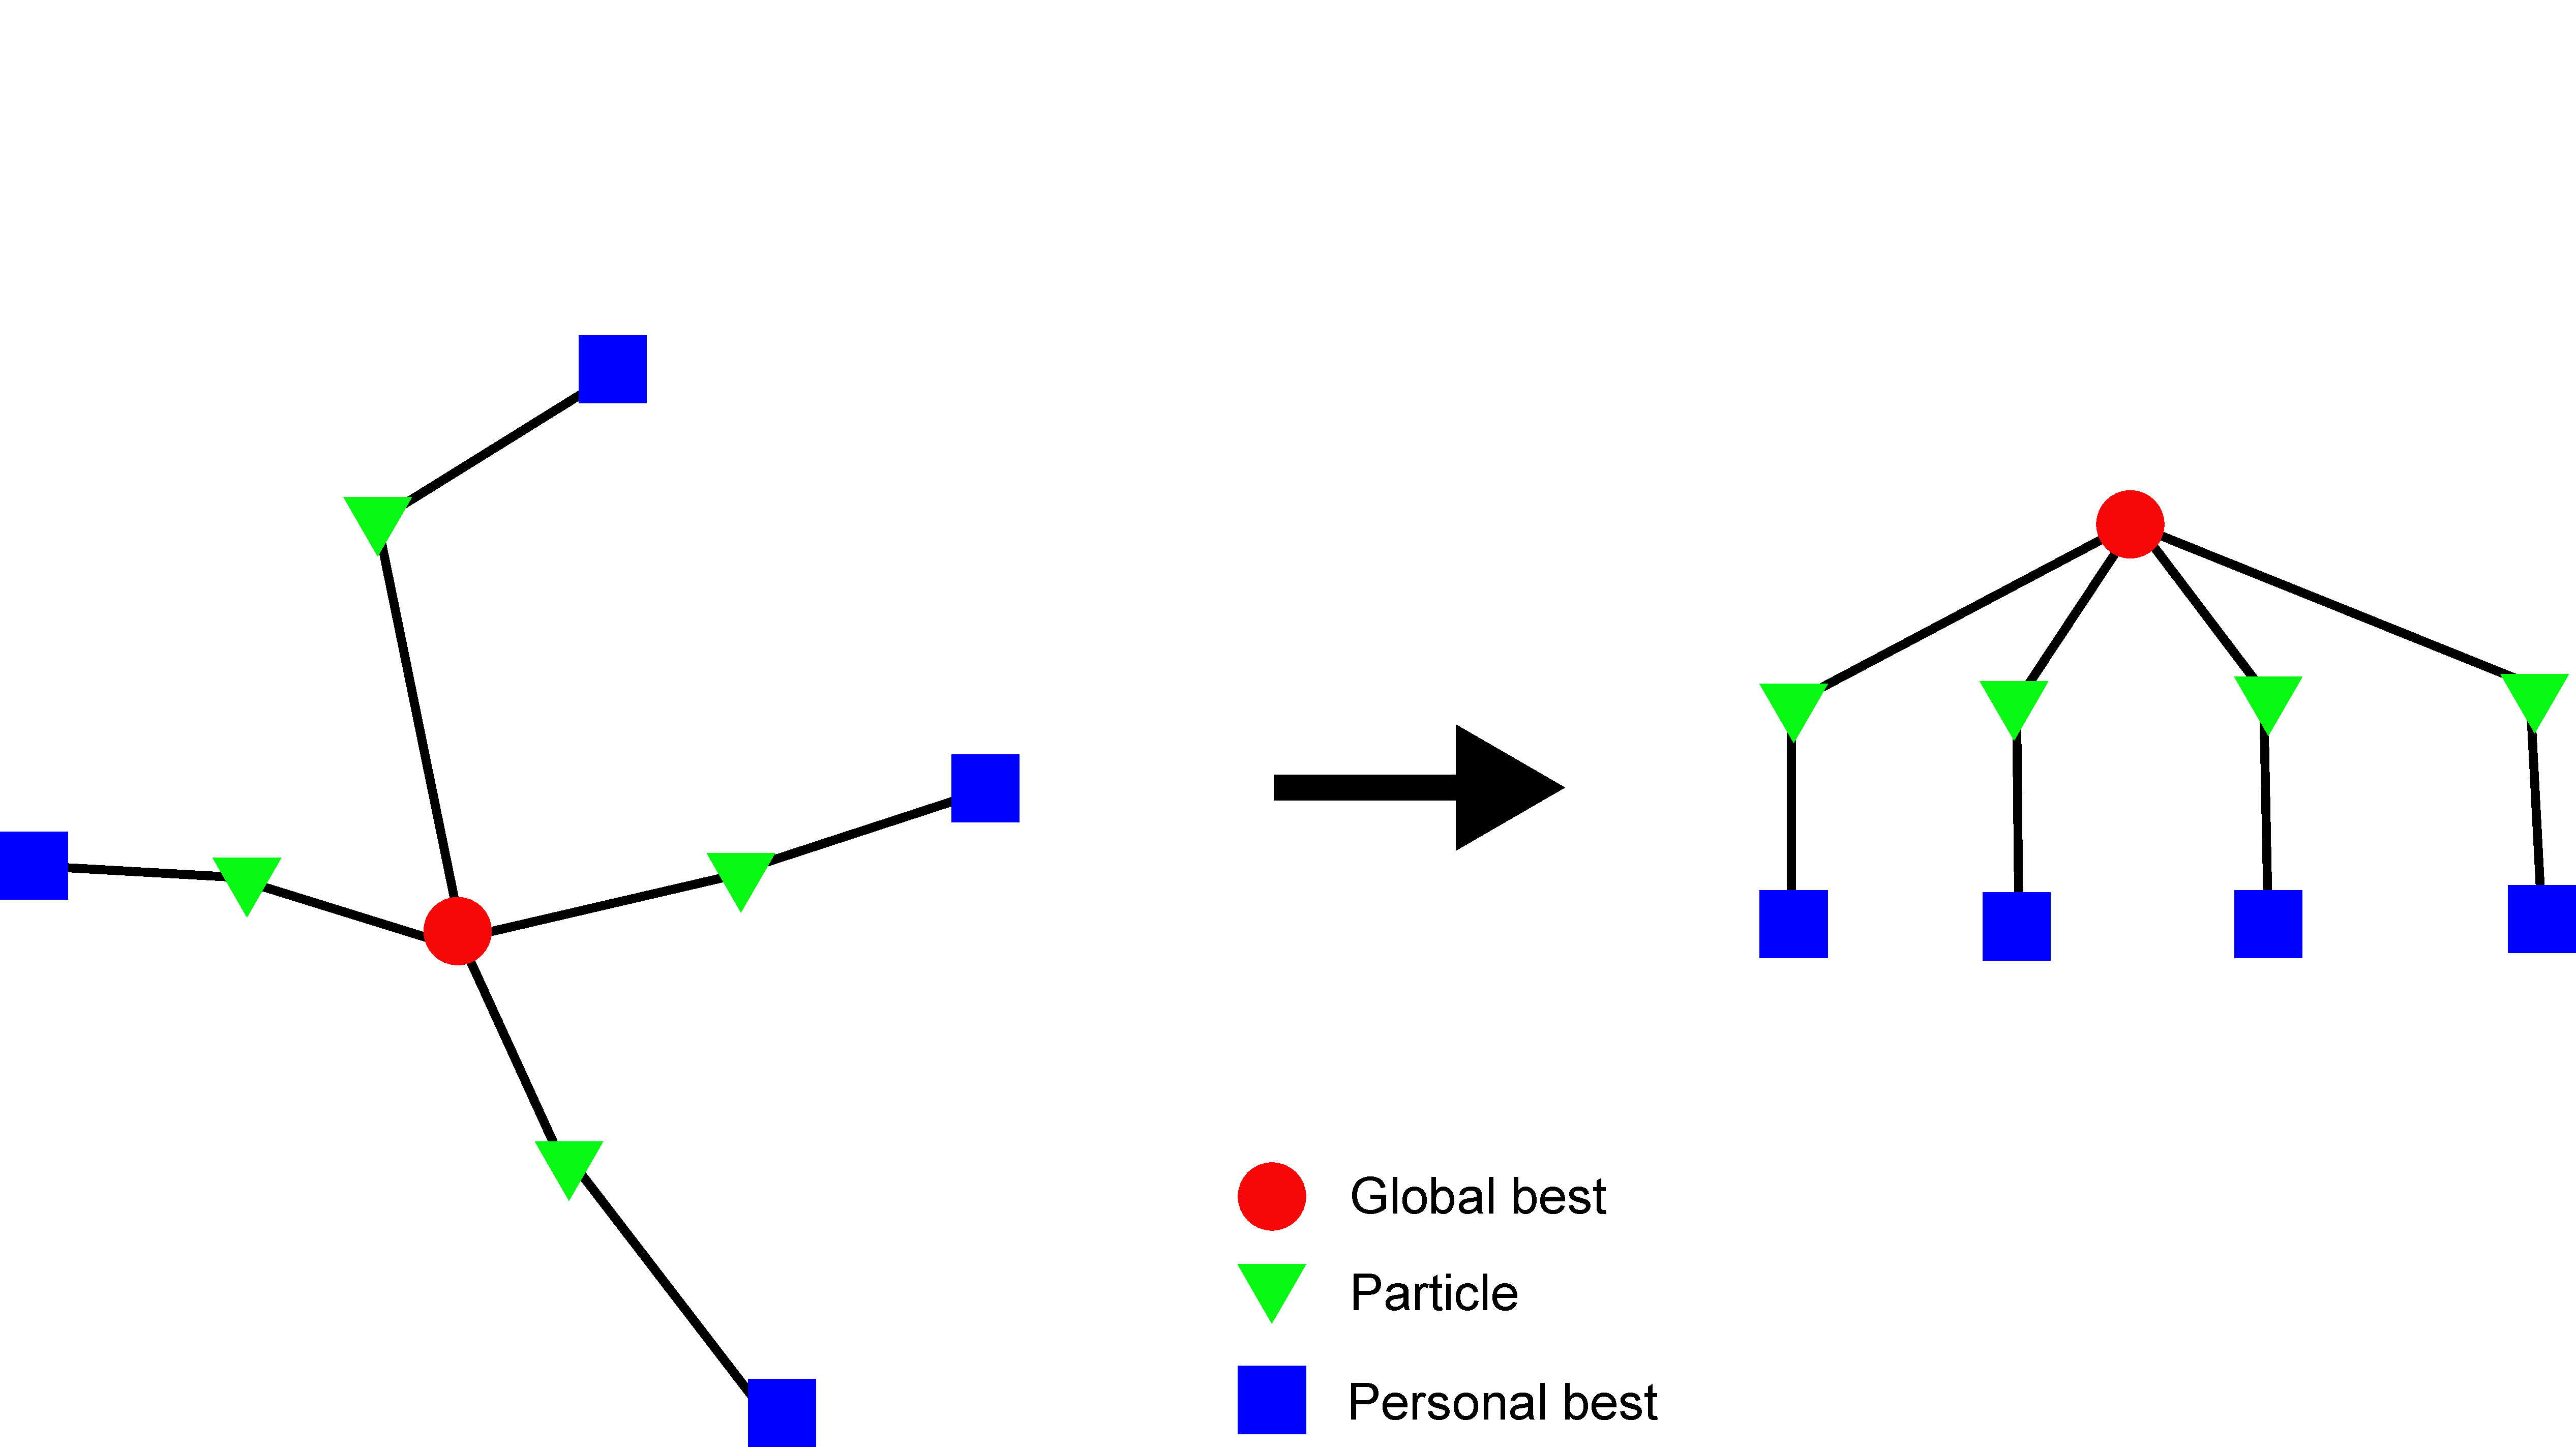
\includegraphics[width=0.7\linewidth]{./topology3}
\caption{The swarm topology}
\label{fig:topology3}
\end{figure}

By this structure, we can see that the interaction between particles are determined by the global best.
It means that when the global best is not changed, the interaction between particles is broken.
If both the global best and personal best are not changed, the interaction between dimensions in a particle is also broken.

\begin{figure}
\centering
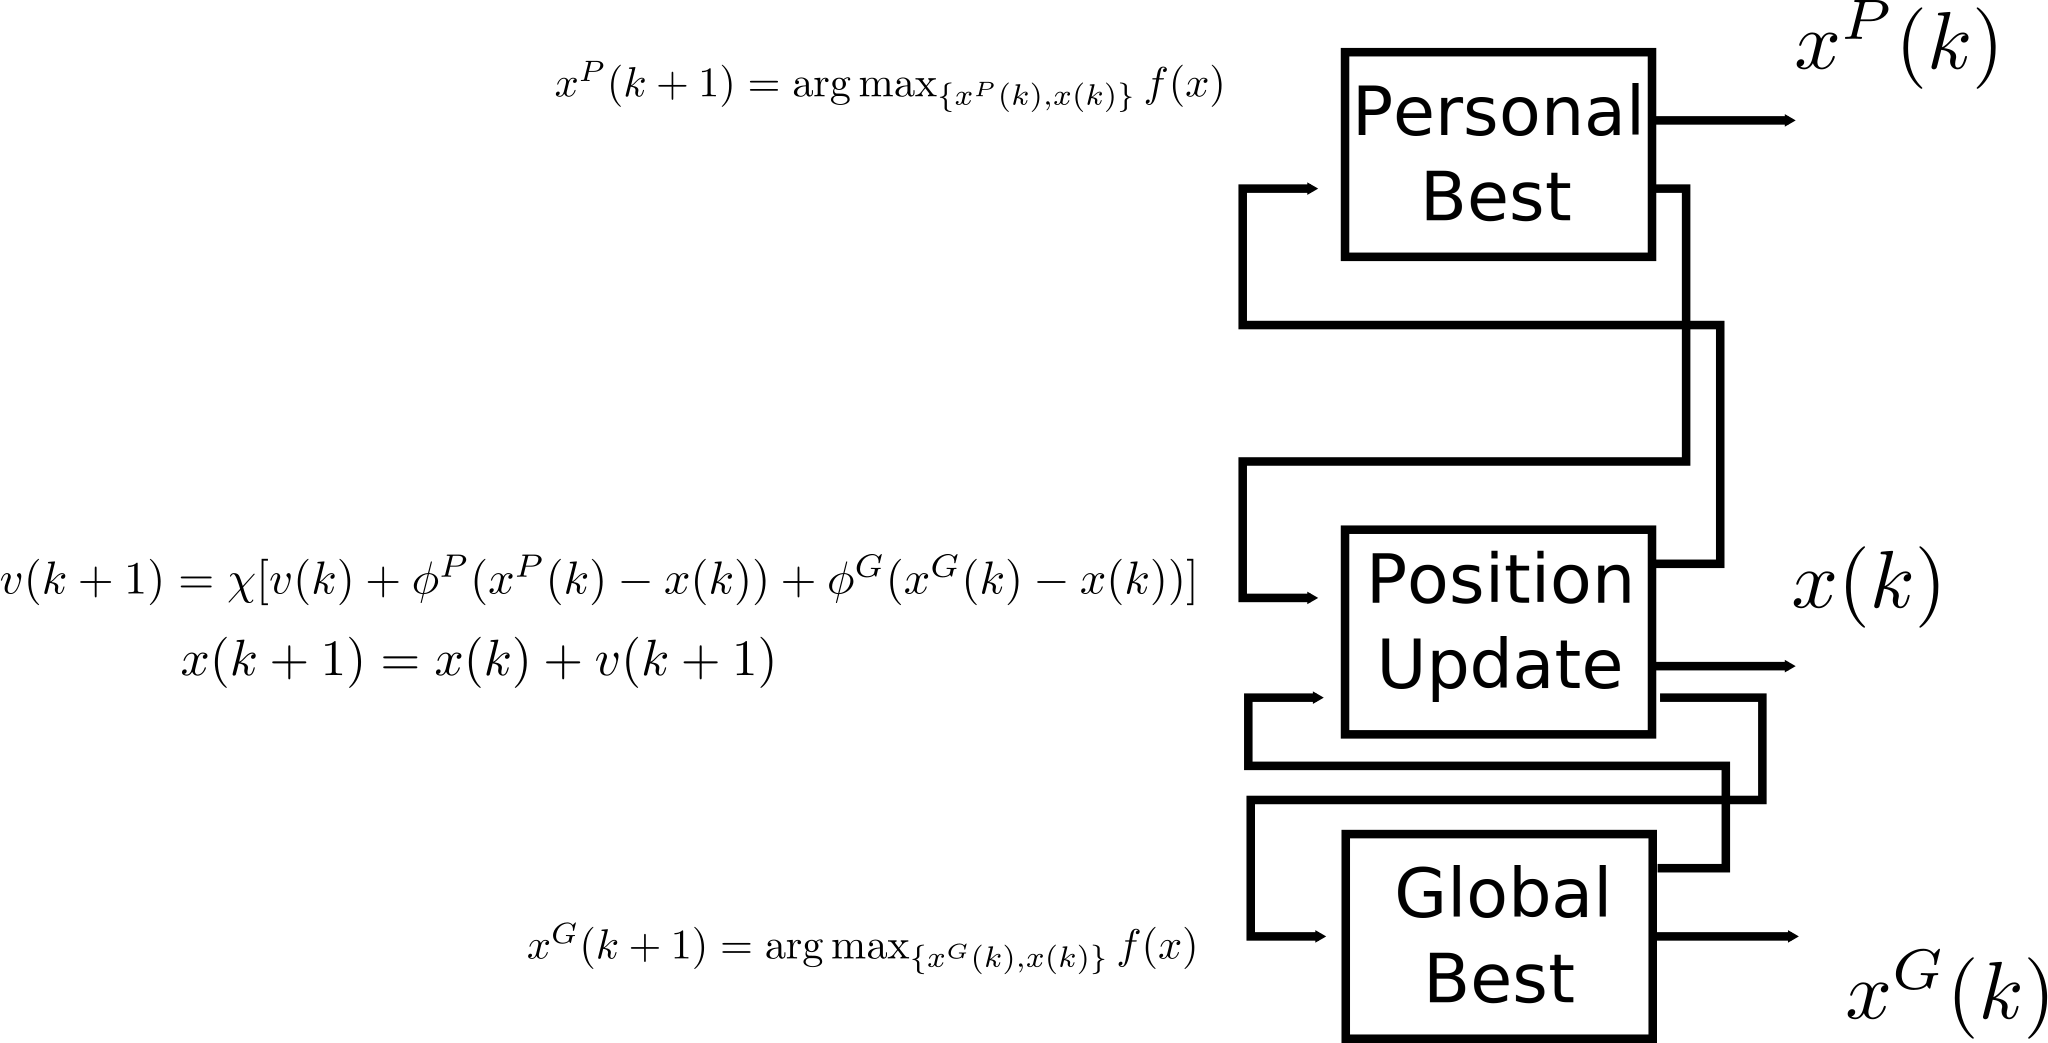
\includegraphics[width=0.9\linewidth]{./structure}
\caption{The interconnection.}
\label{fig:structure}
\end{figure}

\section{Redefine stagnation}

The stagnation phenomenon is usually modeled as that the global best and personal best are not updated.
However, in most of the cases, the personal best might be updated if it is not the same with the global best.
There are two types of situations in the fitness space:
\begin{itemize}
\item global best and personal best are in same hill;
\item global best and personal best are not in same hill.
\end{itemize}

While global best and personal best are in the same hill, the personal best will gradually move toward the global best.

\begin{figure}
\centering
\subfigure[Before updating personal best.] { \label{fig:one_hill_case:a}
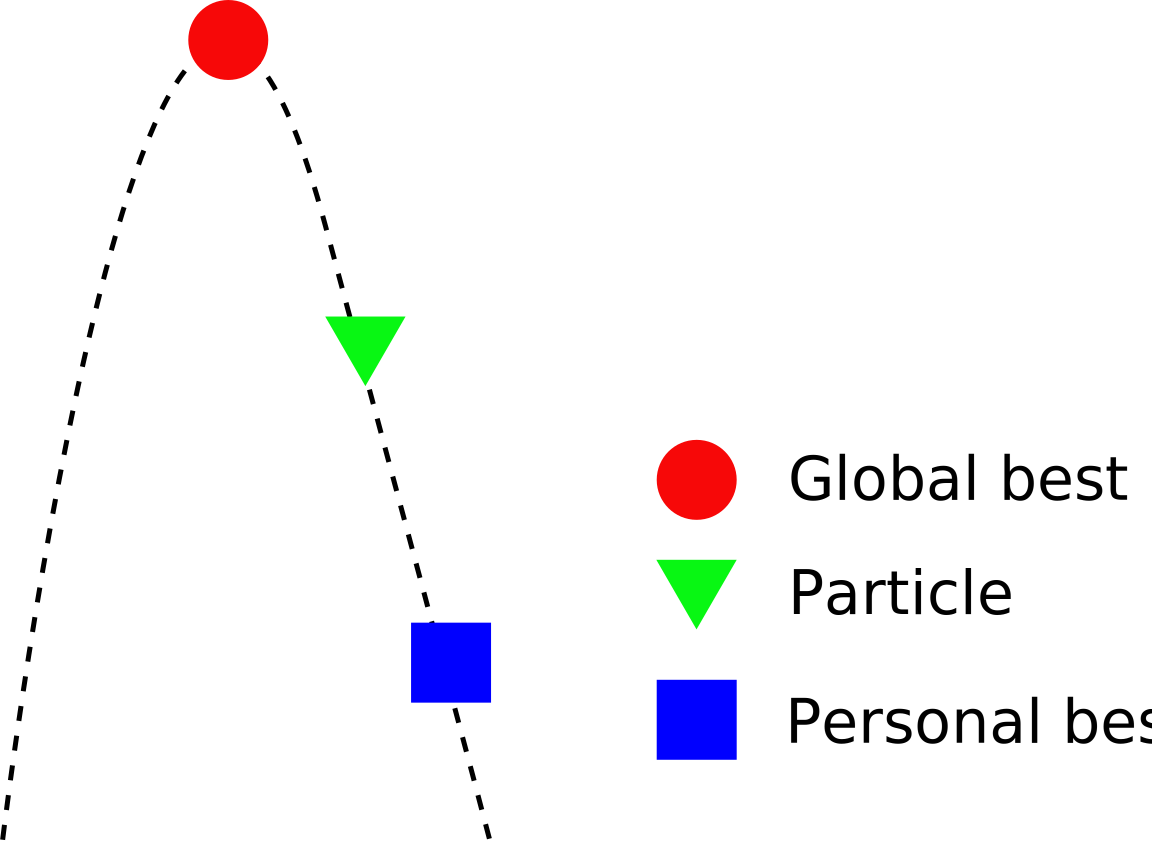
\includegraphics[width=0.47\textwidth]{one_hill_case}
}
\subfigure[After updating personal best.] { \label{fig:one_hill_case:b}
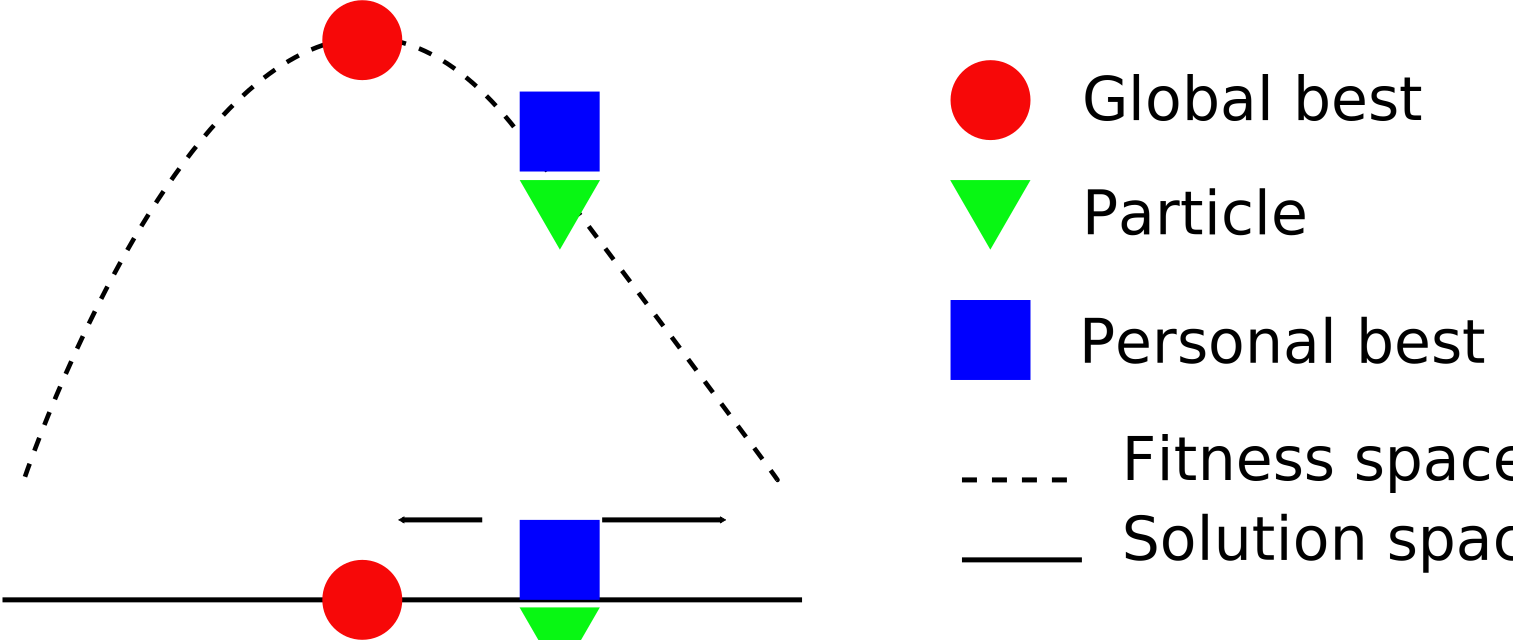
\includegraphics[width=0.47\textwidth]{one_hill_case2}
}
\caption{One hill case.}
\label{fig:one_hill_case}
\end{figure}

When global best and personal best are not in the same hill, the case can be complicated.
There are two cases:
\begin{itemize}
\item the global best is at a hill whose top is higher than that the personal best is at [Figure \ref{fig:two_hills_case:a}];
\item the personal best is at a hill whose top is higher than that the global best is at [Figure \ref{fig:two_hills_case:b}]. 
\end{itemize}
By the moving of a particle, once the global best and the personal best get onto a same hill, it becomes the one hill case in Figure \ref{fig:one_hill_case:b}.
The problem can be answered in two steps:
\begin{itemize}
\item the likelihood that a particle moves a personal best or a global best;
\item the likelihood that a particle converges to a personal best or a global best.
\end{itemize}

\begin{figure}
\centering
\subfigure[The likelihood of moving to the global best.] {\label{fig:two_hills_case:a}
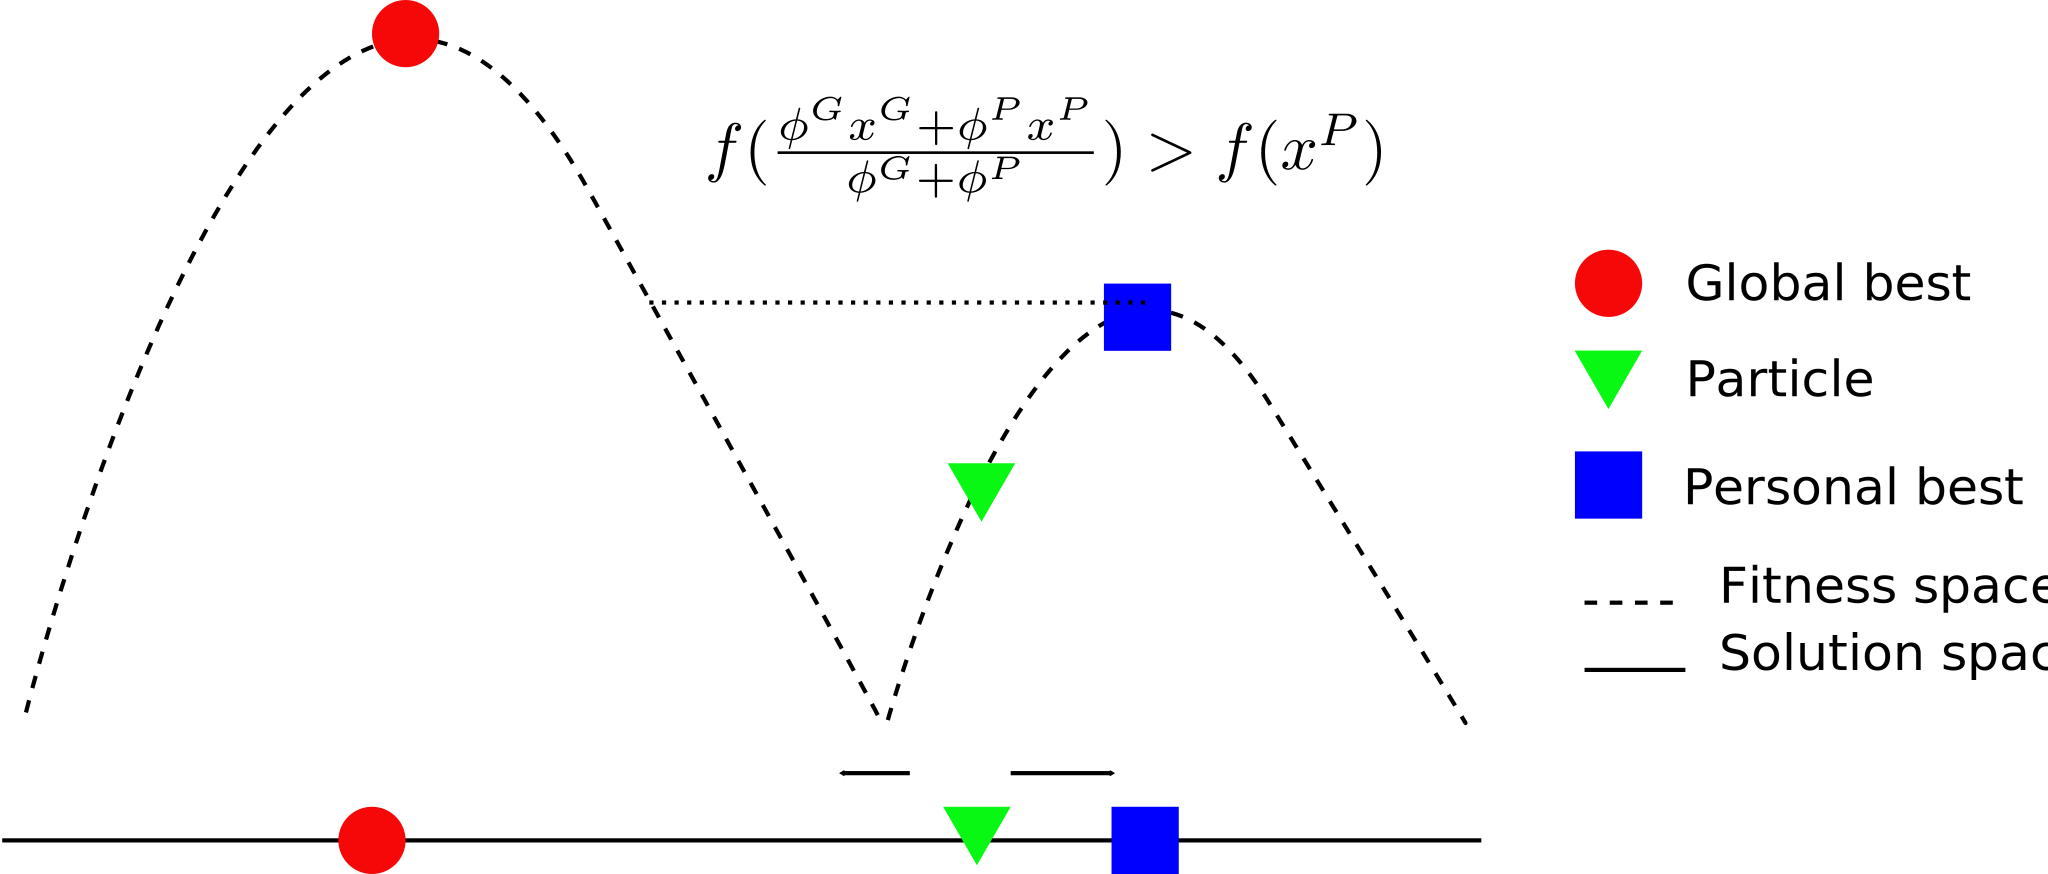
\includegraphics[width=0.57\textwidth]{two_hills_case}
}
\subfigure[The likelihood of moving to the personal best.] {\label{fig:two_hills_case:b}
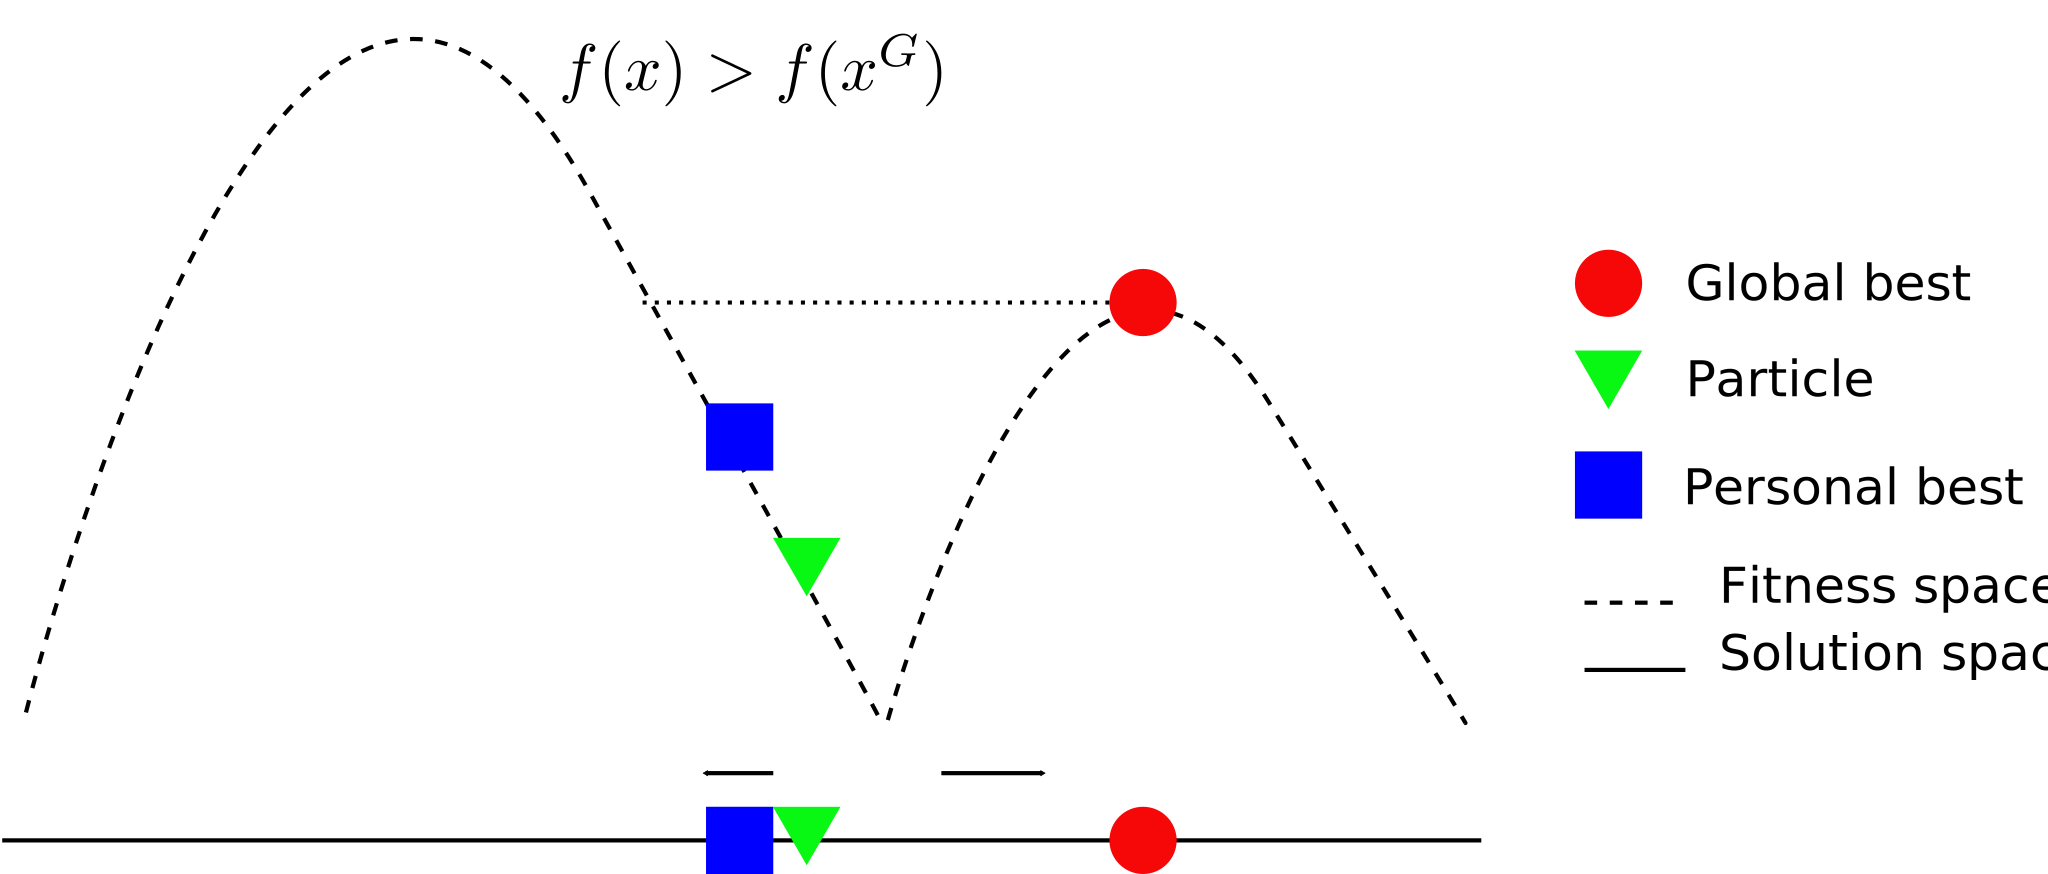
\includegraphics[width=0.57\textwidth]{two_hills_case2}
}
\caption{Two hill case.}
\label{fig:two_hills_case}
\end{figure}


\begin{theorem}
There is a probability $ p $  that a particle moves toward the personal best, and $ 1 - p $ that a particle moves toward the global best,
\begin{equation}
p = 
\end{equation}
\end{theorem}

\begin{corollary}
There is probability $ p $ that the personal best can move to the same hill with the global best,
\begin{equation}
p = 
\end{equation}
\end{corollary}

\section{What happens when the global best is not changed}

\begin{figure}
\centering
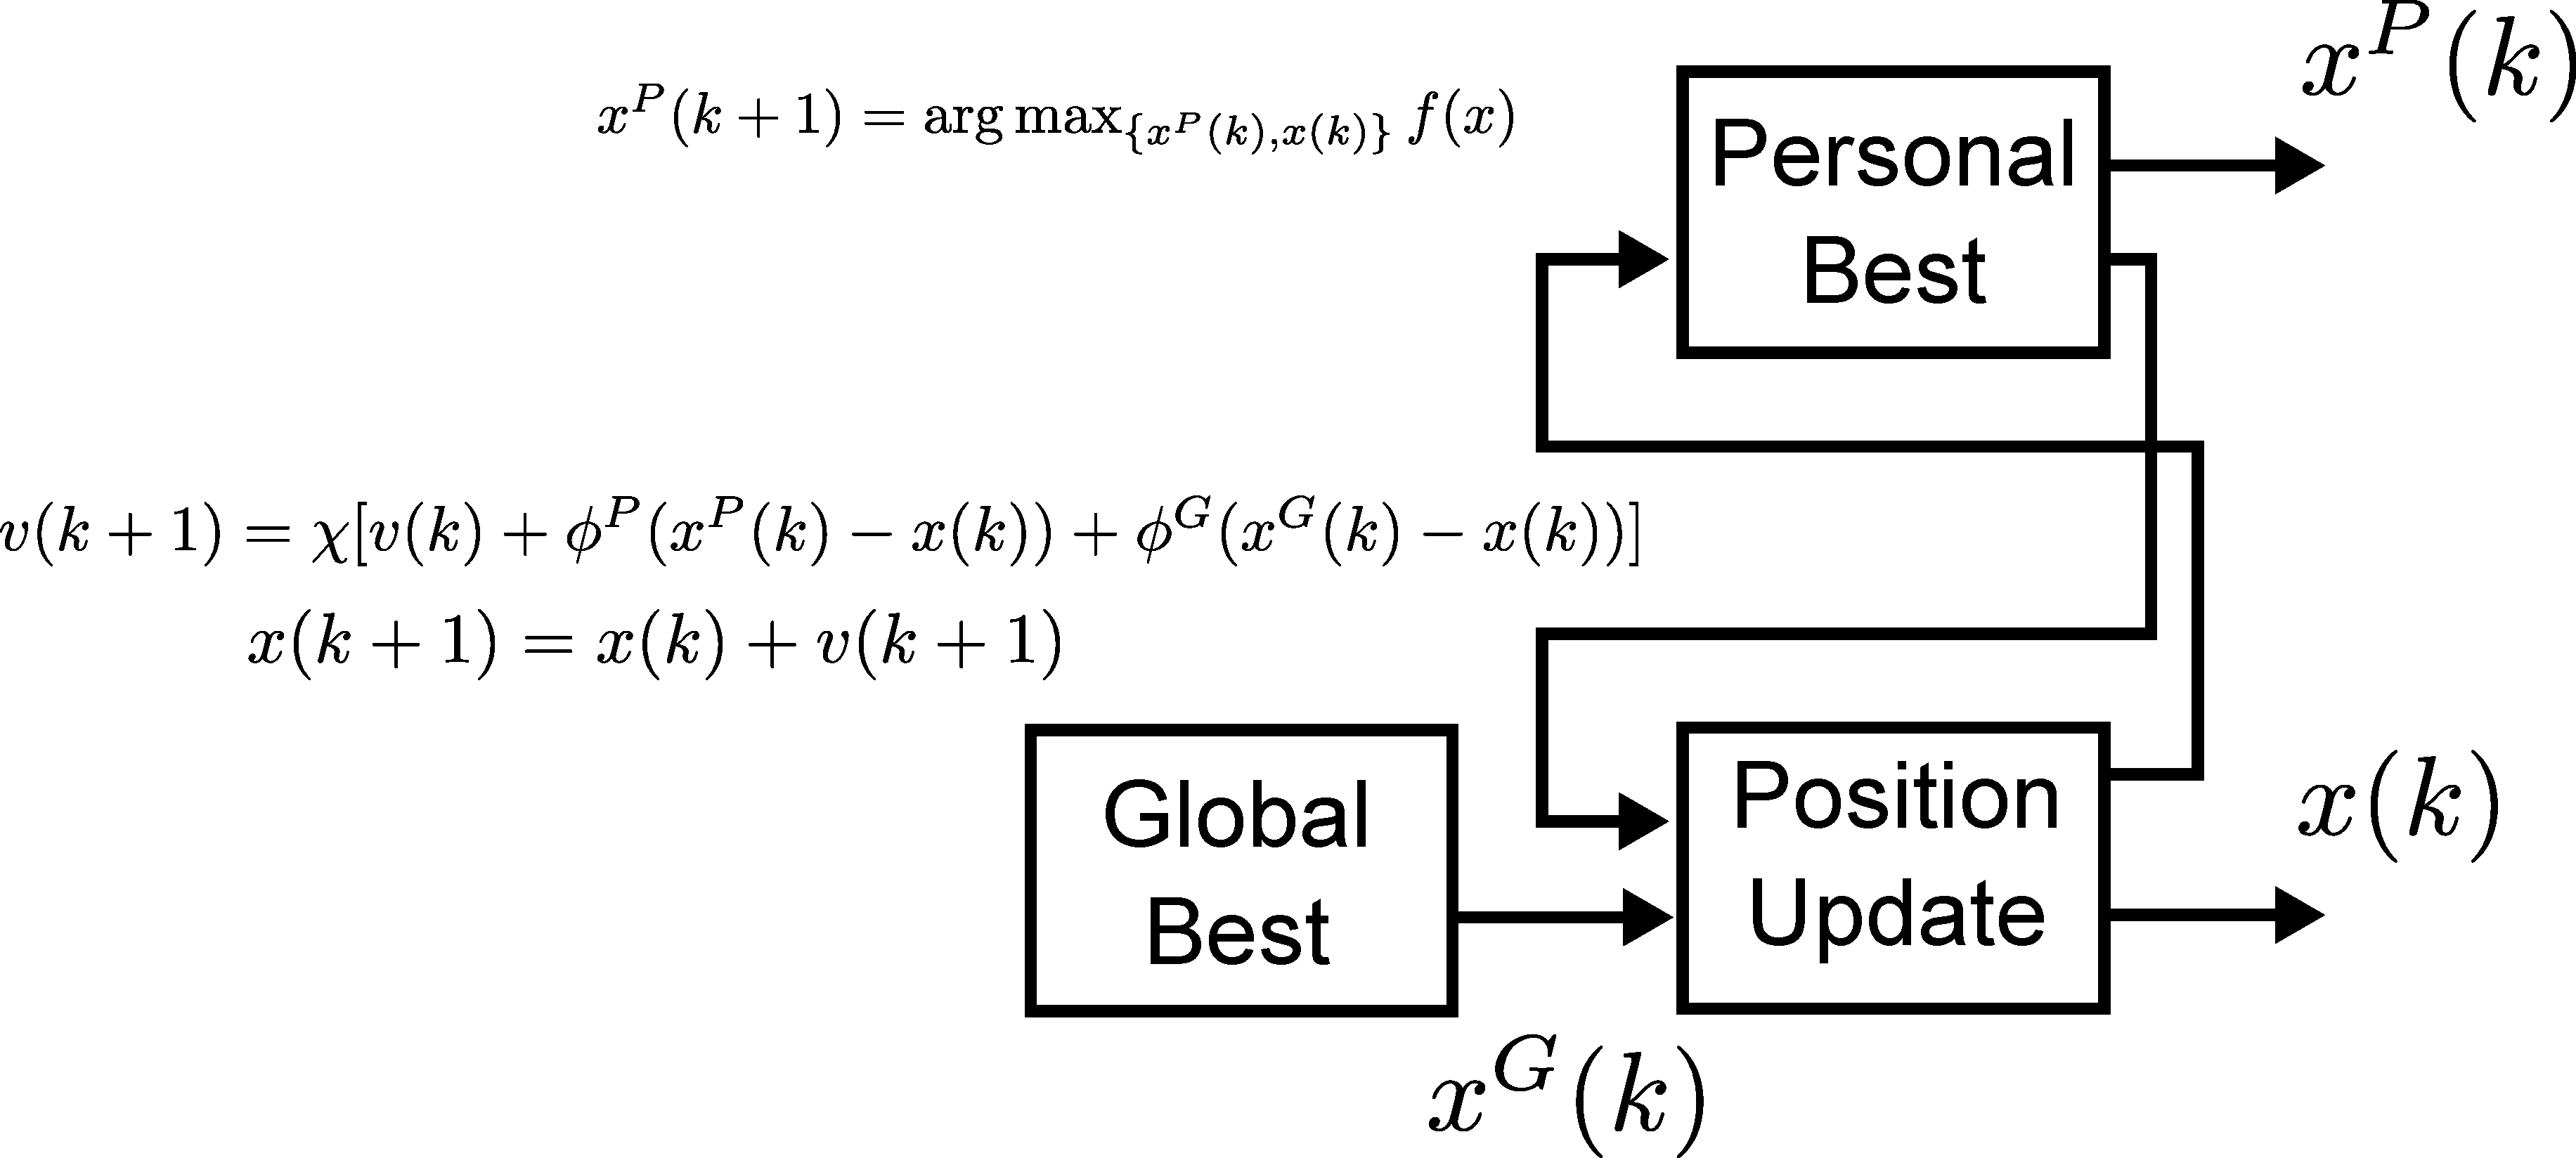
\includegraphics[width=0.8\linewidth]{./structure_constant_gb}
\caption{}
\label{fig:structure_constant_gb}
\end{figure}


Make the global best as the leader

\begin{itemize}
\item 
\item 
\end{itemize}

\section{How a particle is led to a local best or a global best}

This depends on the shape of fitness space


\end{document}